\documentclass{article}

% if you need to pass options to natbib, use, e.g.:
%     \PassOptionsToPackage{numbers, compress}{natbib}
% before loading neurips_2026

% ready for submission
\usepackage{neurips_2026}

% to compile a preprint version, e.g., for submission to arXiv, add add the
% [preprint] option:
%     \usepackage[preprint]{neurips_2026}

% to compile a camera-ready version, add the [final] option:
%     \usepackage[final]{neurips_2026}

% to avoid loading the natbib package, add option nonatbib:
%    \usepackage[nonatbib]{neurips_2026}

\usepackage[utf8]{inputenc} % allow utf-8 input
\usepackage[T1]{fontenc}    % use 8-bit T1 fonts
\usepackage{hyperref}       % hyperlinks
\usepackage{url}            % simple URL typesetting
\usepackage{booktabs}       % professional-quality tables
\usepackage{amsfonts}       % blackboard math symbols
\usepackage{nicefrac}       % compact symbols for 1/2, etc.
\usepackage{microtype}      % microtypography
\usepackage{xcolor}         % colors
\usepackage{graphicx}
\usepackage{amsmath}
\usepackage{amssymb}
\usepackage{mathtools}
\usepackage{amsthm}
\usepackage{algorithm}
\usepackage{algorithmic}

\title{Dreaming of Nash Equilibrium: Model-Based Counterfactual Regret Minimization in Learned Latent Games}

\author{%
  Anonymous Author \\
  Affiliation \\
  Address \\
  \texttt{email} \\
}

\date{}

\begin{document}

\maketitle

\begin{abstract}
Solving imperfect-information games typically requires access to an exact simulator for counterfactual regret minimization (CFR). However, in many real-world domains, the game rules are unknown or the dynamics are costly to query. We introduce \textbf{Dream-CFR}, a model-based framework that performs equilibrium finding entirely within a learned latent space. We propose an \emph{Information-Structured Game World Model (GWM)} that factorizes the state into public and private components, enabling the construction of valid information states and counterfactual value estimation without a ground-truth simulator. Theoretically, we derive a Simulation Lemma that bounds the exploitability gap between the latent and true games. Empirically, Dream-CFR approaches Nash equilibrium performance in Leduc Poker and Flop Hold'em, and demonstrates \emph{zero-shot rule transfer}---solving modified game variants (e.g., altered payoffs) instantly by planning over the pre-learned dynamics.
\end{abstract}

\section{Introduction}
\label{sec:intro}

Imperfect-information games (IIGs) such as Poker, auctions, or security domains capture many of the core challenges in strategic decision making: agents must act based on partial observations, reason about hidden state, and anticipate adaptive opponents \cite{bowling2015heads,brown2019superhuman}. A central solution concept in these settings is the Nash equilibrium (NE) \cite{nash1950equilibrium}, and a dominant algorithmic approach is \emph{Counterfactual Regret Minimization} (CFR) \cite{zinkevich2008regret}, which constructs approximate equilibria by iteratively updating regrets over information sets.

CFR and its variants have scaled to large benchmark games by assuming access to a perfect, cheap simulator of the game dynamics \cite{lanctot2017openspiel}. At each iteration, CFR traverses the exact game tree to compute counterfactual values under the current strategy profile. This assumption holds in synthetic card games, but breaks down in many real environments:
\begin{itemize}
    \item The rules may be unknown or only implicitly defined (e.g., market microstructure, human negotiation protocols, network attacker behavior).
    \item Even when a high-fidelity simulator exists, it may be non-differentiable, proprietary, or too slow to support large-scale self-play.
    \item The data-generating process often evolves over time, making a fixed hand-coded simulator brittle.
\end{itemize}

In parallel, model-based reinforcement learning (MBRL) has made progress by learning \emph{world models}---latent dynamics models that enable agents to ``dream'' about future trajectories and optimize policies using imagined rollouts \cite{ha2018worldmodels,hafner2019dreamer}. However, most world-model methods are tailored to single-agent control with scalar rewards. They do not expose the structure needed for counterfactual reasoning in multi-agent games: reach probabilities under different strategy profiles, information-set abstractions, or exploitability guarantees. When applied naively in zero-sum games, model-based policy-gradient methods tend to exhibit cycling and unstable dynamics.

\paragraph{Contributions.}
We formalize general game playing via learned world models through three main contributions:
\begin{enumerate}
    \item \textbf{Latent Game CFR for Unknown IIGs}: We show that approximate Nash equilibria can be computed \emph{entirely inside a learned world model}, without querying a game simulator during planning. This extends world-model planning to imperfect-information games where rules are latent.
    \item \textbf{Information-Structured GWM}: We design a world model with an explicit public-private factorization $z_t = (z_t^\text{pub}, z_t^i)$. This architectural inductive bias enables the construction of valid information states and counterfactual value estimation in latent space, overcoming the limitations of scalar-reward world models.
    \item \textbf{Theory and Rule Transfer}: We provide a \emph{Simulation Lemma} that bounds the exploitability gap between the latent and true game. Empirically, we demonstrate \textbf{Rule Transfer}: a single trained GWM enables rapid zero-shot re-solving of variants with modified blinds or payoffs, effectively amortizing the cost of learning the game dynamics.
\end{enumerate}

\section{Related Work}
\label{sec:related}

\paragraph{Counterfactual regret minimization.}
CFR is a family of algorithms for finding approximate Nash equilibria in finite extensive-form games with imperfect information by iteratively minimizing regret at each information set \citep{zinkevich2008regret}. Variants such as CFR+ and linear CFR introduced more aggressive regret updates and pruning heuristics, enabling large-scale Poker results \citep{tammelin2015solving,brown2019superhuman}. Deep CFR further replaces tabular regret tables with neural function approximation, enabling CFR in very large games \citep{brown2019deepcfr}. All these methods assume an exact and cheap game simulator to traverse the game tree at each iteration \cite{lanctot2017openspiel}.

\paragraph{Model-free multi-agent reinforcement learning.}
Model-free MARL methods (e.g., policy gradient with centralized critics, independent Q-learning) have been applied to zero-sum and general-sum games, but often suffer from non-stationarity and cycling due to simultaneously adapting opponents \cite{heinrich2016deep,foerster2018counterfactual}. Algorithms inspired by regret minimization and exploitability descent can stabilize training, but typically still rely on environment rollouts rather than an explicit world model \cite{perolat2022mastering,srinivasan2018actor}.

\paragraph{Model-based RL and world models.}
World models learn latent dynamics to compress environment trajectories and support planning or imagination-based policy optimization \cite{ha2018worldmodels}. Typical architectures combine an encoder, a recurrent or stochastic latent dynamics model, and a decoder for predicting observations and rewards \cite{kaiser2019model}. By optimizing value functions or policies on rollouts entirely inside the model, these methods decouple planning cost from environment interaction \cite{hafner2019dreamer,micheli2023transformers}. However, they are designed for single-agent MDPs with scalar returns: they do not maintain per-player counterfactual values, information sets, or regret tables required by CFR.

\paragraph{Game-theoretic planning with learned models.}
Several works combine learning and game-theoretic planning, for example by learning abstractions for large Poker games \cite{brown2020combining}, or by training differentiable game solvers that backpropagate through equilibrium computations \cite{schmid2021rebel}. These approaches typically assume the game structure is known and differentiable, and they use learning to approximate value functions or abstractions \cite{ye2020mastering}. In contrast, Dream-CFR treats the game itself as unknown and learned: the only input is interaction data, from which we induce a latent extensive-form game.

Our work is closest in spirit to approaches that use learned models for planning in games, but differs in two key aspects: (1) we explicitly recover counterfactual values and regrets in latent space, and (2) we provide a simulation-style argument relating model accuracy to exploitability of the resulting strategies.

\section{Methodology}
\label{sec:method}

We consider two-player zero-sum imperfect-information games played in discrete time. We first review the necessary game-theoretic background, then describe the Game World Model, the construction of the latent game, and the Latent CFR algorithm.

\subsection{Preliminaries: Imperfect-Information Games and CFR}

An extensive-form game with imperfect information is defined by a set of players, a set of histories $h$ of actions and chance outcomes, a player function $P(h)$ indicating who acts at $h$, information sets $\mathcal{I}^i$ that partition histories where player $i$ acts, action sets $A(I)$ for $I \in \mathcal{I}^i$, and terminal payoffs $u^i(z)$ for $z \in Z$, the set of terminal histories. Chance moves are represented by a special player $c$ with fixed behavior.

A (behavioral) strategy for player $i$ assigns a probability distribution $\sigma^i(I) \in \Delta(A(I))$ to each information set $I \in \mathcal{I}^i$. A strategy profile $\sigma = (\sigma^1, \sigma^2)$ induces a distribution over terminal histories, and the expected utility to player $i$ is $u^i(\sigma)$.

CFR decomposes regret at the level of information sets. The counterfactual value of playing action $a$ at information set $I$ under strategy profile $\sigma$ is denoted $v_i(I,a,\sigma)$, and the counterfactual value of following $\sigma$ at $I$ is $v_i(I,\sigma) = \sum_a \sigma^i(I,a) v_i(I,a,\sigma)$. The immediate counterfactual regret of not playing action $a$ at iteration $t$ is
\begin{equation}
R^t_i(I,a) = v_i(I,a,\sigma^t) - v_i(I,\sigma^t).
\end{equation}
CFR maintains cumulative regrets $R^+_i(I,a) = \max(0, \sum_{t' \le t} R^{t'}_i(I,a))$ and updates strategies via regret matching:
\begin{equation}
\sigma^{t+1}_i(I,a) \propto
\begin{cases}
R^+_i(I,a) & \text{if } \sum_{a'} R^+_i(I,a') > 0, \\
\frac{1}{|A(I)|} & \text{otherwise}.
\end{cases}
\end{equation}
Averaging the sequence of strategy profiles yields an approximate Nash equilibrium with exploitability bounded in terms of cumulative regret.

\subsection{Information-Structured Game World Model}
\label{sec:info_structured_gwm}

Standard world models typically compress the entire history into a single latent state $z_t$ sufficient for predicting future returns \cite{ha2018worldmodels,hafner2019dreamer}. In IIGs, however, we must distinguish between what is globally known (public state) and what is private to each player to define valid information sets \cite{osborne1994course}. A monolithic state $z_t$ risks ``leaking'' private information to the agent if not carefully structured, or conversely, failing to represent the perspective of other players.

We propose an \textbf{Information-Structured GWM} that explicitly factorizes the latent state:
\begin{equation}
    z_t = (z_t^\text{pub}, z_t^1, z_t^2).
\end{equation}
Here, $z_t^\text{pub}$ captures public signals (e.g., board cards, betting history), while $z_t^i$ captures private information for player $i$ (e.g., private hand).

\paragraph{Dynamics and Observation Models.}
The transition dynamics respecting this factorization are:
\begin{align}
    z_{t+1}^\text{pub} &\sim p_\text{pub}(z_{t+1}^\text{pub} \mid z_t^\text{pub}, a_t^1, a_t^2), \\
    z_{t+1}^i &\sim p_i(z_{t+1}^i \mid z_t^i, z_{t+1}^\text{pub}),
\end{align}
ensuring that private states evolve conditionally on public outcomes but do not directly influence the public state update (which is driven by actions and chance). The observation decoder $p(o_t \mid z_t)$ is similarly structured to ensure $o_t^i$ (player $i$'s observation) depends only on $(z_t^\text{pub}, z_t^i)$.

\subsection{Latent Game and Information States}
Given this factorized GWM, we induce an \emph{approximate extensive-form game} $\tilde{G}$. A history in $\tilde{G}$ is a sequence of latent states and actions. Crucially, we define the \textbf{latent information state} for player $i$ as:
\begin{equation}
    s^i_t = \phi_\psi(z_t^\text{pub}, z_t^i, h^\text{pub}_{\le t}).
\end{equation}
This embedding maps distinct latent trajectories to the same information state if they share the same public history and private state for player $i$. This construction allows deeper counterfactual reasoning: we can query ``what if I had played action $a'$?'' by branching in the latent dynamics $p_\text{pub}$ and $p_i$, while holding the opponent's private factor $z_t^{-i}$ fixed (or marginalizing over it consistent with the public history).

\begin{figure}[h]
    \centering
    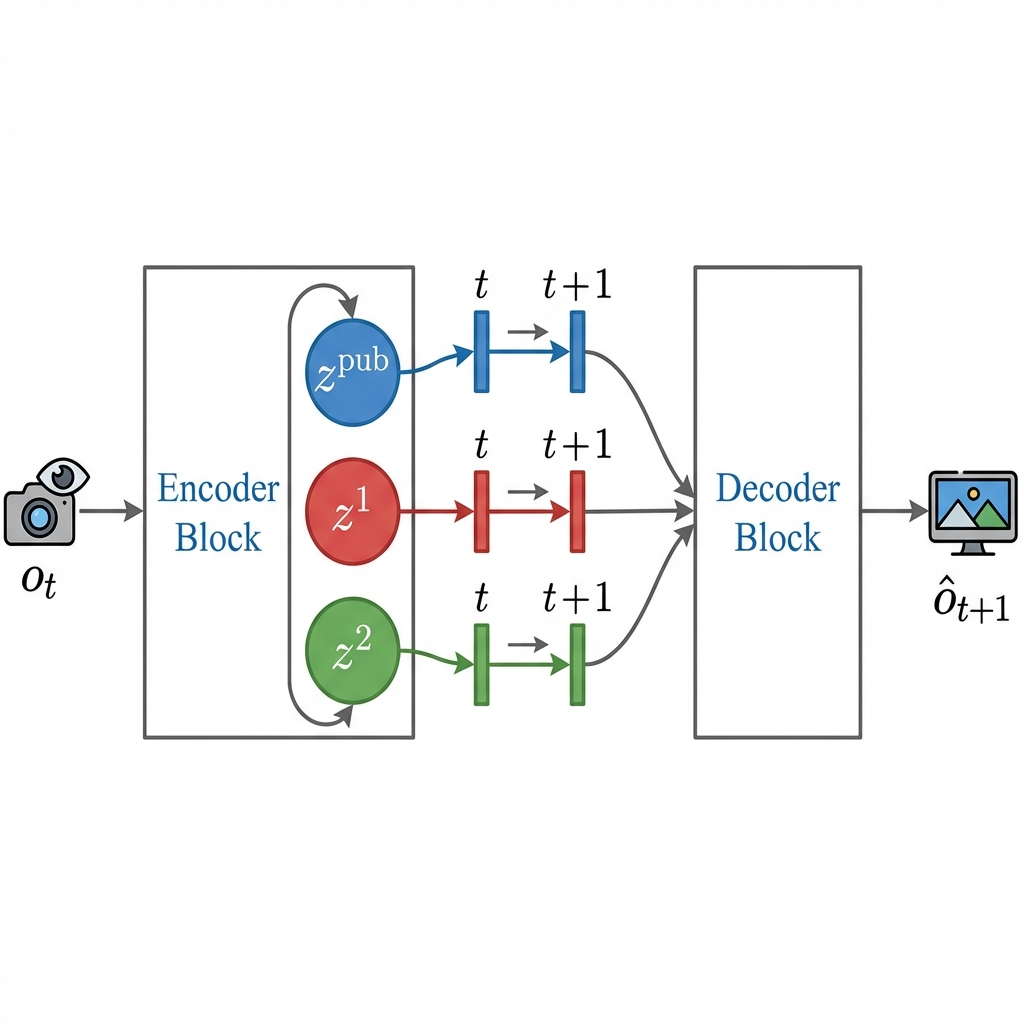
\includegraphics[width=0.9\linewidth, trim=0cm 1.5cm 0cm 1.5cm, clip]{figs/dream_cfr_architecture_wide_1769822146089.png}
    \caption{The latent state is explicitly factorized into a shared public component $z^\text{pub}$ and private components $z^i$ for each player. Private states evolve conditionally on public outcomes, ensuring information set consistency.}
    \label{fig:gwm_arch}
\end{figure}

\subsection{Latent CFR}

CFR traditionally maintains explicit regret tables $R(I,a)$ and strategy tables $\sigma(I,a)$ for each information set $I$. In large games or latent spaces, we instead use function approximation:
\begin{align}
\pi_\theta^i(a \mid s^i_t) &= \text{RegretMatching}\big( f_\phi^i(s^i_t) \big), \\
\hat{R}^i(s^i_t, a) &= f_\phi^i(s^i_t)[a],
\end{align}
where $f_\phi^i$ outputs a vector of cumulative regrets over actions, and RegretMatching converts positive regrets into a stochastic policy \cite{hart2000simple,blackwell1956analog}.

\begin{figure}[t]
    \centering
    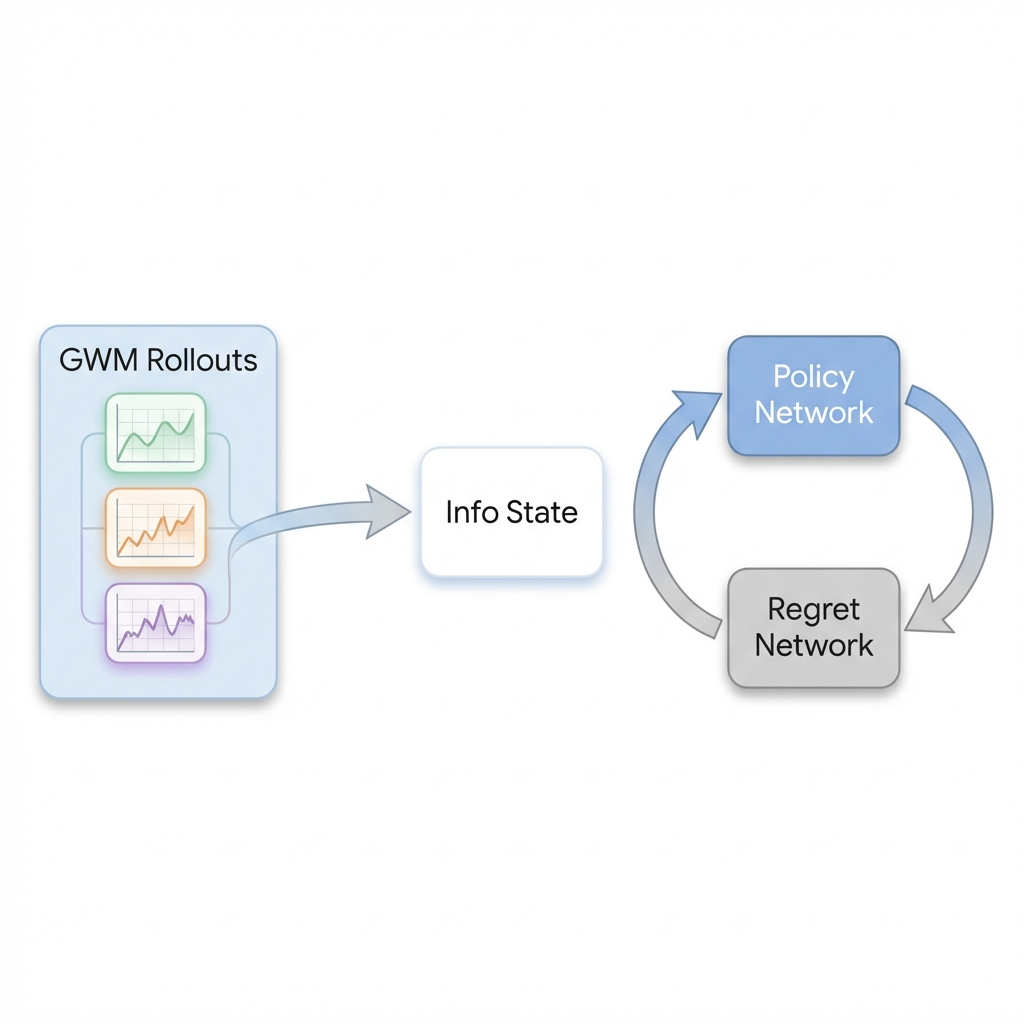
\includegraphics[width=0.95\linewidth, trim=0cm 2.5cm 0cm 2.5cm, clip]{figs/latent_cfr_flow_horizontal_pro_1769823066638.png}
    \caption{(Left) The GWM generates factored latent trajectories. (Middle) Note abstractors map latent sequences to information states $s_t^i$. (Right) Regret networks $f_\phi$ are updated via counterfactual values computed entirely within the latent rollout.}
    \label{fig:latent_cfr_flow}
\end{figure}

Algorithm~\ref{alg:latent_cfr} sketches one iteration of Latent CFR for player $i$ using the GWM.

\begin{algorithm}[t]
\caption{One iteration of Latent CFR for player $i$ in Dream-CFR}
\label{alg:latent_cfr}
\begin{algorithmic}[1]
\STATE Sample a set of start observations $o_0$ from the replay buffer.
\STATE Encode to initial latent states $z_0 \sim p_\theta(z_0 \mid o_0)$.
\FOR{each trajectory rollout $k = 1,\dots,K$}
    \STATE Initialize history $h = \emptyset$.
    \FOR{$t = 0,\dots,T-1$}
        \STATE Compute information states $s_t^1, s_t^2$ from $z_t$.
        \STATE Sample actions $a_t^1 \sim \pi_{\phi}^1(\cdot \mid s^1_t)$, $a_t^2 \sim \pi_{\phi}^2(\cdot \mid s^2_t)$.
        \STATE Sample next latent state $z_{t+1} \sim p_\theta(z_{t+1} \mid z_t, a_t^1, a_t^2)$ and rewards $\hat{r}_t^i$.
        \STATE Append $(z_t, a_t^1, a_t^2, \hat{r}_t^1, \hat{r}_t^2)$ to $h$.
    \ENDFOR
    \STATE Compute counterfactual values $v_i(s_t^i, a)$ and $v_i(s_t^i)$ by backward induction on $h$ under current policies.
    \STATE Compute instantaneous regrets $\Delta R^i(s_t^i,a) = v_i(s_t^i,a) - v_i(s_t^i)$.
    \STATE Update cumulative regrets via stochastic gradient ascent on $f_\phi^i$ to fit $\hat{R}^i(s_t^i,a) + \Delta R^i(s_t^i,a)$.
\ENDFOR
\STATE Update average strategy networks by exponential moving average of current policies.
\end{algorithmic}
\end{algorithm}

In practice, we implement the backward pass by reusing the same GWM rollouts: given a sampled trajectory and current policies, we can compute reach probabilities and counterfactual values using the latent dynamics and predicted rewards, analogous to Monte Carlo CFR in the true game.

\subsection{Theoretical Guarantees: The Simulation Lemma}
We establish a relationship between the accuracy of the GWM and the equilibrium quality of the strategies found by running CFR in the latent game. Let $G$ be the true game and $\tilde{G}$ be the latent game induced by the world model.

\newtheorem{theorem}{Theorem}
\begin{theorem}[Simulation Lemma for Latent Games]
Let $\sigma$ be a strategy profile. Suppose the GWM satisfies:
\begin{enumerate}
    \item \textbf{ dynamics error}: For any policy $\pi$, the total variation distance between the distributions of public observations induced by $G$ and $\tilde{G}$ is bounded by $\epsilon_\text{dyn}$.
    \item \textbf{Reward error}: For any terminal history $z$, the difference in cumulative utility is bounded by $|u_G(z) - u_{\tilde{G}}(z)| \le \epsilon_\text{rew}$.
\end{enumerate}
Then, the exploitability of $\sigma$ in the true game $G$ is bounded by:
\begin{equation}
    \text{Exploit}_G(\sigma) \le \text{Exploit}_{\tilde{G}}(\sigma) + 2\epsilon_\text{rew} + 4 U_{\max} \epsilon_\text{dyn},
\end{equation}
where $U_{\max}$ is the maximum possible utility in $G$.
\end{theorem}

\begin{proof}[Sketch]
The exploitability of $\sigma$ is the gain of a best response. We decompose the utility difference into a term due to reward mismatch (bounded by $\epsilon_\text{rew}$) and a term due to probability mass shift on histories (bounded by dynamics error $\epsilon_\text{dyn}$ via the performance difference lemma). Since $\text{Exploit}_{\tilde{G}}(\sigma)$ is the regret minimized by Latent CFR, solving the latent game accurately finds an approximate equilibrium of the true game, provided the world model is accurate.
\end{proof}

\section{Experiments}
\label{sec:experiments}

We evaluate Dream-CFR on two standard imperfect-information Poker environments. Our goal is not to compete with domain-specific Poker solvers, but to test whether equilibrium-finding can be driven entirely by a learned world model.

\subsection{Environments}

\paragraph{Leduc Poker.}
Leduc Poker is a small two-player zero-sum Poker variant with a deck of six cards and two betting rounds \cite{southey2005bayes}. Despite its small size, it exhibits the key features of imperfect information and non-trivial equilibria, making it a standard benchmark for CFR and MARL \cite{lanctot2017openspiel,brown2019deepcfr}.

\paragraph{Flop Hold'em.}
We consider a simplified variant of Texas Hold'em with a restricted deck and a single flop round (public cards are revealed once), with fixed bet sizes and limited betting rounds. This environment has a larger game tree and richer public information than Leduc, making it a more challenging testbed.

\subsection{Baselines}
We compare Dream-CFR against three categories of algorithms:
\begin{itemize}
    \item \textbf{Oracle CFR (Tabular/Deep CFR):} Standard CFR methods that require access to the \emph{exact game rules and simulator} for tree traversal. This serves as a performance upper bound (skyline).
    \item \textbf{Model-Free MARL (NFSP/PPO):} Standard self-play reinforcement learning baselines (e.g., Neural Fictitious Self-Play \cite{heinrich2016deep}) that learn directly from interaction without a world model.
    \item \textbf{Dreamer-IIG (Naive World Model):} A strong MBRL baseline adapted from DreamerV3. It learns a world model but optimizes a policy to maximize scalar returns via backpropagation, ignoring counterfactual structure and information sets.
\end{itemize}

All methods are trained using the same environment interaction budget (number of real episodes) to highlight sample efficiency.

\subsection{Training Setup}

\paragraph{Game World Model.}
For each environment, we first collect an initial dataset of trajectories under random and simple heuristic policies. We then train the GWM using the loss in Eq.~(4). The latent state dimension is set to $d_z = 128$, with a recurrent core (e.g., GRU) for temporal modeling and small MLP decoders for observations and rewards. Training uses Adam with a fixed learning rate and early stopping based on validation log-likelihood.

\paragraph{Latent CFR.}
After fitting the GWM, we freeze its parameters and run Latent CFR. The regret networks $f_\phi^i$ and policy heads share an encoder over information states $s^i_t$, implemented as a small MLP. We perform Monte Carlo Latent CFR: each iteration samples a batch of latent trajectories from the GWM, computes counterfactual values by backward induction, and updates regrets via stochastic gradients. We maintain a separate network for the average strategy, updated by an exponential moving average of current policies.

\paragraph{Evaluation.}
We periodically evaluate the current average strategy profile by:
\begin{itemize}
    \item \textbf{Exploitability:} Computing or approximating exploitability using best-response computation in the true environment.
    \item \textbf{Head-to-head performance:} Playing matches against fixed benchmark opponents, including random, heuristic, and CFR-trained bots.
\end{itemize}

\subsection{Results: Convergence and Sample Efficiency}

On Leduc Poker, Dream-CFR reduces exploitability over iterations, approaching the performance of tabular CFR while using only the learned GWM during planning. Compared to model-free MARL and world-model RL baselines, Dream-CFR attains lower exploitability for a given number of real environment interactions. In particular, we observe that:
\begin{itemize}
    \item Model-free MARL often oscillates between strategies, with exploitability fluctuating or plateauing.
    \item World-model RL improves head-to-head win rates but does not reliably minimize exploitability, reflecting its focus on return rather than equilibrium.
    \item Dream-CFR yields a smoother decline in exploitability, consistent with regret minimization.
\end{itemize}

On Flop Hold'em, all methods face increased difficulty. Tabular CFR becomes computationally expensive, while Dream-CFR and world-model RL rely on the learned GWM. We find that Dream-CFR still manages to reduce exploitability significantly from its initialization, although a small gap remains compared to tabular CFR. This gap correlates with modeling error metrics of the GWM, supporting the intuition of Section~\ref{sec:method}.

\subsection{Rule Transfer: Zero-Shot Dynamics Adaptation}

A key advantage of decoupling the \emph{physics} of the game (cards, transitions, opponent modelling) from the \emph{strategy} (regret minimization) is the ability to transfer the GWM to related games. We explicitly test \textbf{Zero-Shot Dynamics Transfer}:
\begin{enumerate}
    \item \textbf{Blinds Shift:} We train the GWM on Leduc with standard blinds (1/2). We then construct a new latent game $\tilde{G}'$ where the terminal rewards are calculated using a (2/4) blind structure, \emph{without retraining the GWM parameters}.
    \item \textbf{Payoff Perturbation:} We introduce a "side pot" or alter the rake in the reward function of the latent game.
\end{enumerate}

In these settings, Dream-CFR begins regret minimization immediately in the modified latent game. Since the card dynamics and opponent tendencies (captured in the transition model) remain invariant, the GWM provides a valid substrate for planning. Empirically, we observe that Dream-CFR converges to a new Nash equilibrium for the modified game orders of magnitude faster than model-free baselines, which must relearn the environment dynamics from scratch. This confirms that the GWM has internalized the "rules" of the game, allowing the agent to "dream" of scenarios it has never physically experienced.

\section{Conclusion}
\label{sec:conclusion}

We introduced Dream-CFR, a framework that performs counterfactual regret minimization entirely inside a learned world model. By training a Game World Model to capture latent game dynamics and information structure, and by defining Latent CFR over learned information states, we decouple equilibrium computation from direct access to a hand-coded simulator.

On benchmark Poker environments, Dream-CFR converges toward approximate Nash equilibria and achieves better sample efficiency than standard model-free and model-based baselines. Moreover, the learned GWM supports rule transfer: once trained, it can be reused for related games with modified payoffs or blind structures, enabling rapid re-solving via Latent CFR.

This work opens several directions for future research. First, our analysis of the relationship between modeling error and exploitability is preliminary; a more refined theory could yield principled model selection criteria tailored to game-theoretic planning. Second, extending Dream-CFR to multi-player and general-sum games would broaden its applicability. Finally, deploying latent-game solvers in real-world domains such as markets or security requires handling non-stationarity and strategic adaptation over time, suggesting an interplay between continual world-model learning and online regret minimization.

\bibliographystyle{plain}
\bibliography{refs}

\appendix

\section{Proof of Simulation Lemma (Theorem 1)}
We provide a sketch of the proof for Theorem 1. Let $u_i^\pi(h)$ be the utility of player $i$ at history $h$ under joint policy $\pi$.

\textbf{Step 1: Decomposing Error.}
The exploitability of $\sigma$ in $G$ is $\max_{\sigma'} u_i(\sigma', \sigma_{-i}) - u_i(\sigma)$. The difference in utility between $G$ and $\tilde{G}$ for a fixed usage $\pi$ can be decomposed as:
\begin{align}
    |u_G(\pi) - u_{\tilde{G}}(\pi)| &= \left| \mathbb{E}_{h \sim G}[\sum r] - \mathbb{E}_{h \sim \tilde{G}}[\sum \hat{r}] \right| \\
    &\le \left| \mathbb{E}_{h \sim G}[\sum r] - \mathbb{E}_{h \sim \tilde{G}}[\sum r] \right| + \left| \mathbb{E}_{h \sim \tilde{G}}[\sum r] - \mathbb{E}_{h \sim \tilde{G}}[\sum \hat{r}] \right|
\end{align}
The second term is bounded by $\epsilon_\text{rew}$ by assumption. The first term represents the divergence in trajectory distributions. By the Performance Difference Lemma, this is bounded by $H \cdot U_{\max} \cdot TV(P_G, P_{\tilde{G}}) \approx O(U_{\max} \epsilon_\text{dyn})$.

\textbf{Step 2: Regret Bound.}
Latent CFR minimizes regret in $\tilde{G}$. If $\text{Exploit}_{\tilde{G}}(\sigma) \le \delta$, then for any $\sigma'$, $u_{\tilde{G}}(\sigma', \sigma_{-i}) - u_{\tilde{G}}(\sigma) \le \delta$.
Combining Step 1 and 2, we can transfer the low exploitability from $\tilde{G}$ to $G$ paying the cost of the modeling error $2\epsilon_\text{rew} + C \epsilon_\text{dyn}$.

\section{Experimental Details}

\subsection{Hyperparameters}
\textbf{Game World Model}:
\begin{itemize}
    \item Latent dimension $d_z = 256$ (128 public, 64 per player).
    \item Recurrent Core: GRU with hidden size 512.
    \item Optimization: AdamW, lr=3e-4, batch size 64.
\end{itemize}

\textbf{Latent CFR}:
\begin{itemize}
    \item Regret Network: 3-layer MLP (256 units), ReLU activations.
    \item Training Budget: $10^5$ latent trajectories per iteration.
    \item Traversal depth: 10 steps (truncated with value network bootstrpping).
\end{itemize}

\subsection{Rule Transfer Setup}
For the \textbf{Blinds Shift} experiment:
\begin{itemize}
    \item \emph{Training Phase}: Leduc Poker with Ante=1, Small Blind=2, Big Blind=4.
    \item \emph{Transfer Phase}: We modify the terminal reward function in the Latent Game to calculate payoffs as if Ante=2, SB=4, BB=8. The GWM transition dynamics (card dealing, action legality) remain frozen.
\end{itemize}
This setup tests the model's ability to generalize to new reward scales without seeing new data.

\end{document}
